\documentclass[xcolor=table]{beamer}
% Just load the xcolor with the options table in the \documentclass. Because beamer loads by default xcolor package, therefore, it is necessary to pass the options in the \documentclass.

\mode<presentation>
{
  \usetheme{CambridgeUS}      % or try Darmstadt, Madrid, Warsaw, ...
  \usecolortheme{default} % or try albatross, beaver, crane, ...
  \usefonttheme{default}  % or try serif, structurebold, ...
  \setbeamertemplate{navigation symbols}{}
  \setbeamertemplate{caption}[numbered]
} 

\usepackage[english]{babel}
\usepackage[utf8x]{inputenc}

\title[Méthodes d'analyses quantitatives]{\textbf{SOC2206} \\
Introduction aux méthodes d'analyses quantitatives et computationnelles en Sociologie \\
\textbf{Introduction et présentation du cours}}

\author{Vissého Adjiwanou, Ph.D}

\institute[Sociologie]{\bf Département de Sociologie, UQAM}
%\textsc {Industrial Training Presentation }


\date{$6^{\text{th}}$ September 2018}

\begin{document}

\begin{frame}
  \titlepage
\end{frame}


\section{Plan de la présentation}

\begin{frame}{Plan de la présentation}

\begin{itemize}
  	\item Introduction 
  	\begin{itemize}
  	    \item Qui suis-je?
  	    \item Changements majeurs dans l'enseignement des statistiques
  	\end{itemize}
    \item Description du cours
	\item Objectifs
	\item Matériels
	\item Mode d'évaluation
	\item Calendrier
    \item Inspiration
    
\end{itemize}

% Commands to include a figure:
%\begin{figure}
%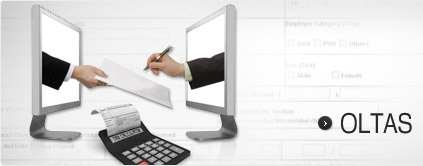
\includegraphics[width=5cm ,height= 3cm]{oltas-header.jpg}
%\caption{\label{fig:your-figure}OLTAS}
%\end{figure}
%\vskip 1cm

\end{frame}
%%%%%%%%%%%%%%%

\section{Qui suis-je?}

\begin{frame}{Parcours}

\begin{itemize}
  \item Parcours académique et professionnel sur trois continents
  \item Précédemment professeur à la \textit{University of Cape Town (South Africa)}.
  

\end{itemize}

% Commands to include a figure:

\begin{figure}
\centering
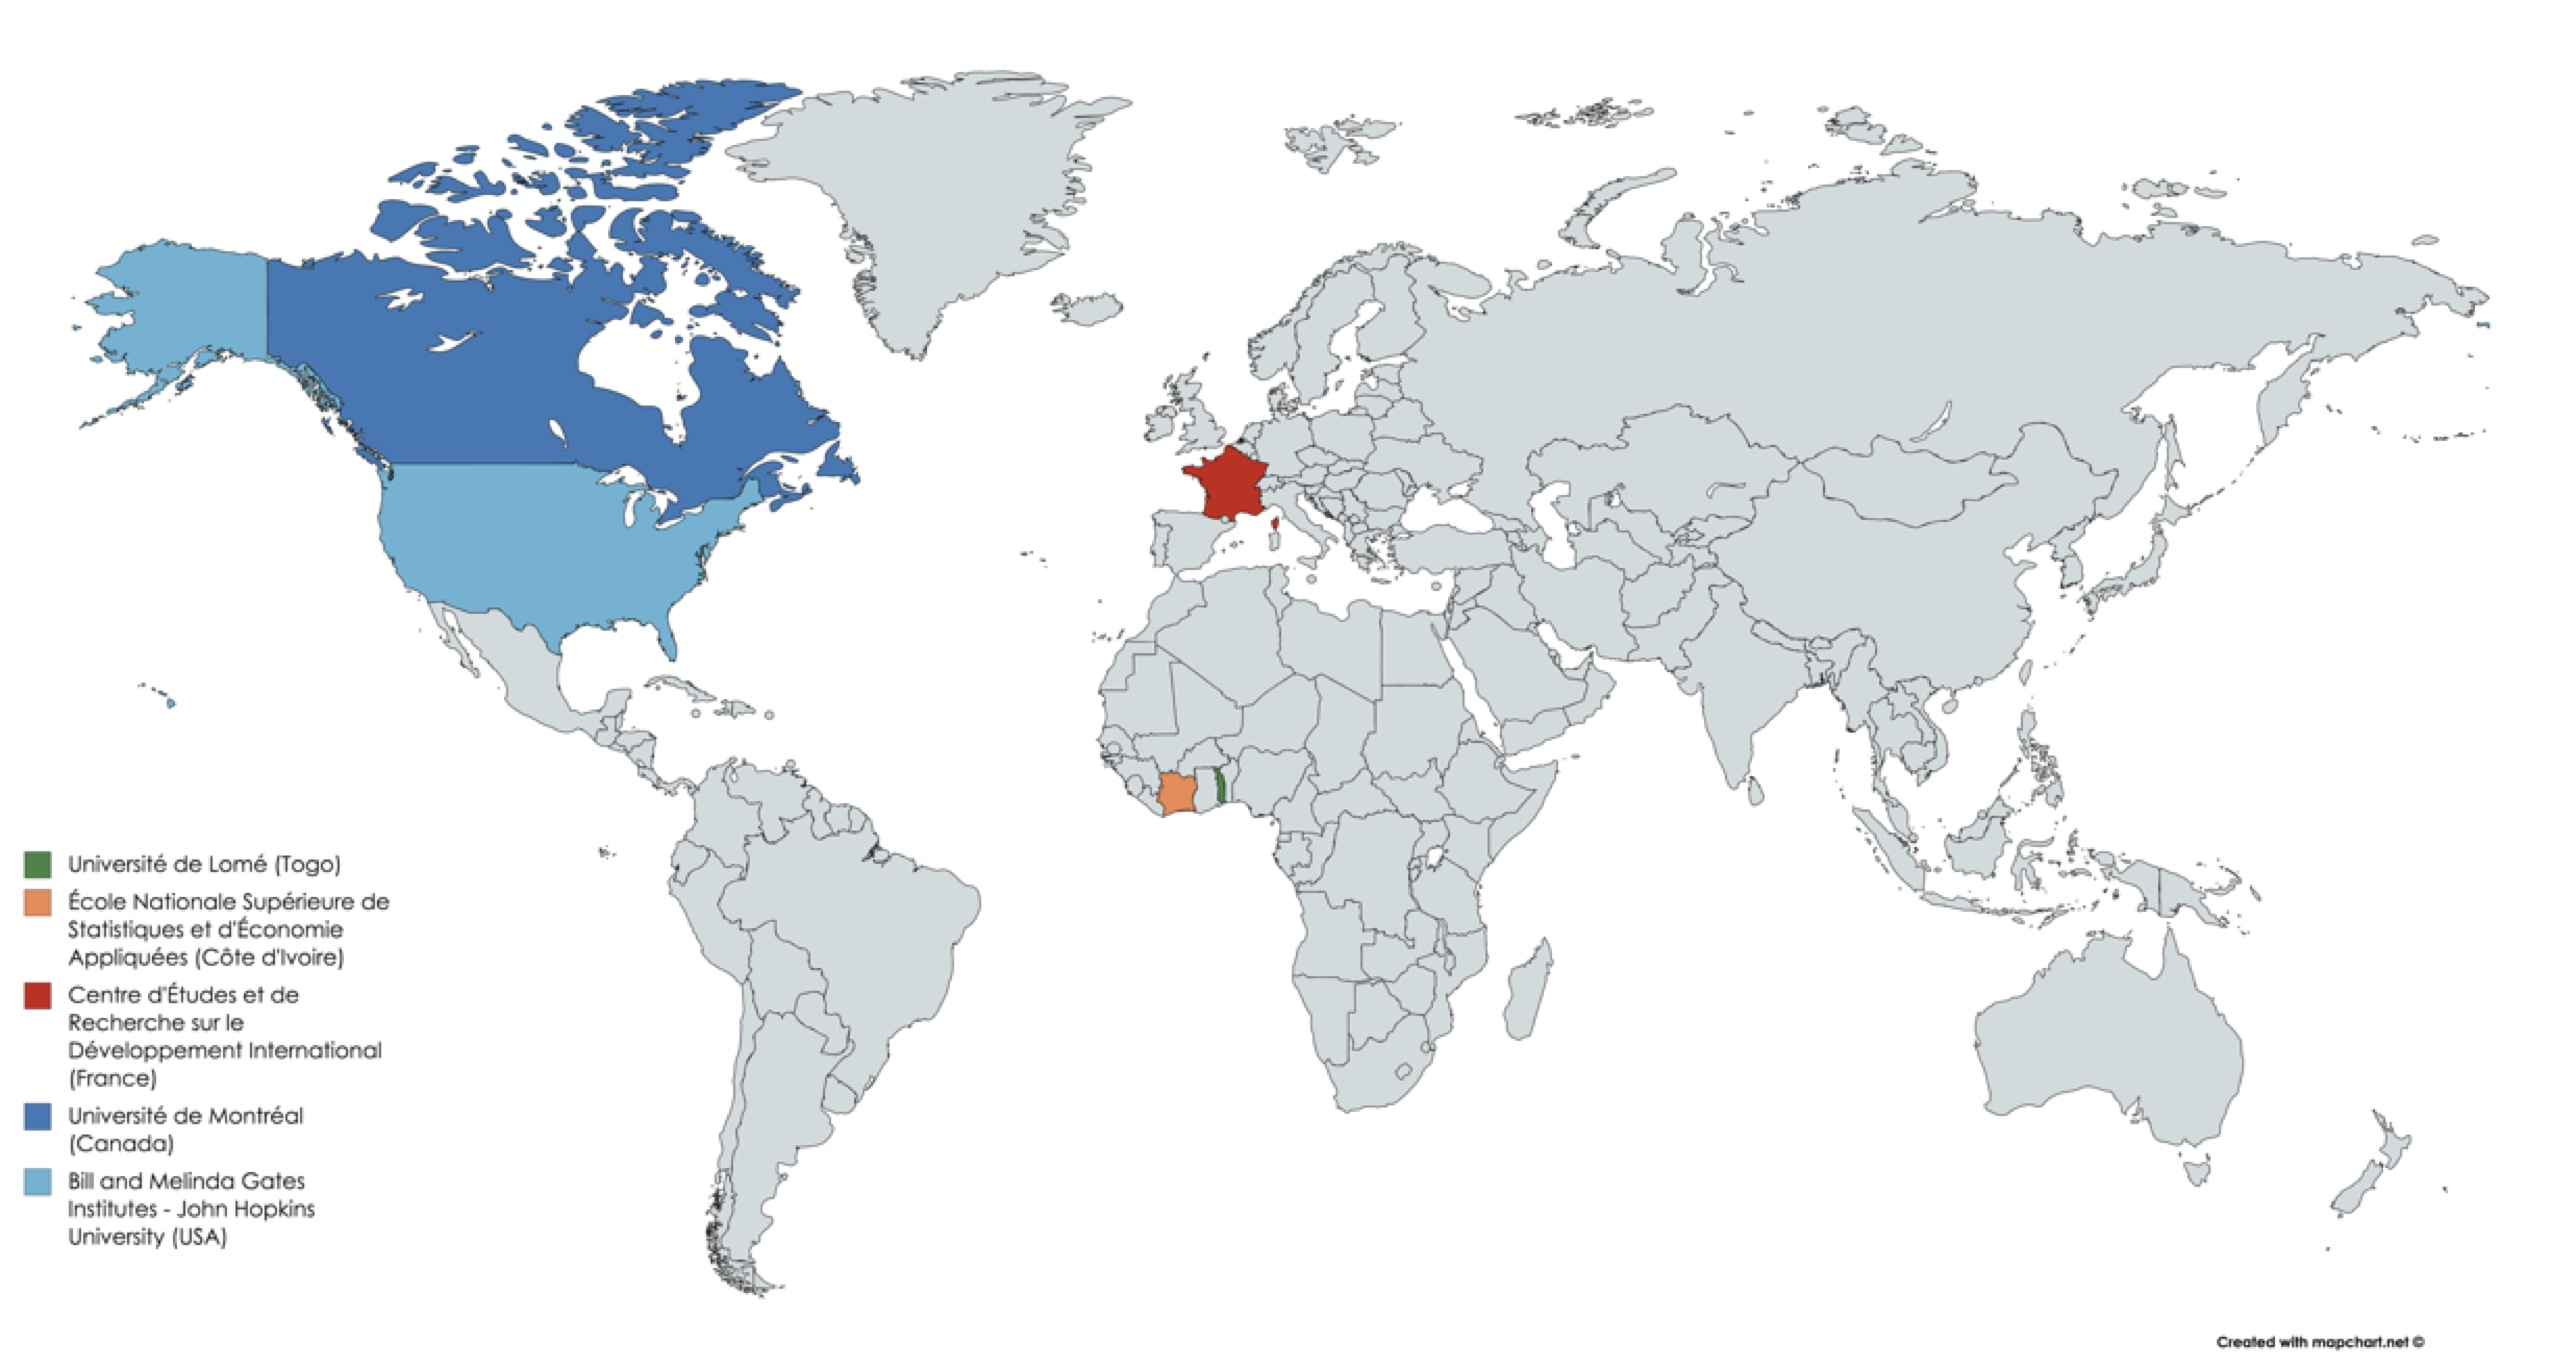
\includegraphics[width=10cm ,height= 5cm]{Parcours.jpg}
\caption{\label{fig:your-figure}Parcours académique et professionnel}
\end{figure}
\vskip 1cm

\end{frame}

%%%%%%%%%%%%%%%

\section{Qui suis-je?}

\begin{frame}{Formations et expériences}

\begin{itemize}
  \item Doctorat en Démographie, Université de Montréal
  \item Maîtrise en économie du développement, Centre d'Études et de Recherche sur le Développement International (CERDI), France
  \item Ingénieur des Travaux Statistiques, École Nationale de Statistiques et d'Économie Appliquées (ENSEA), Côte d'Ivoire
  \item Diplôme de mathématiques, Université de Lomé (Togo)

\end{itemize}

\vskip 1cm
\end{frame}

%%%%%%%%%%%%%%%

\begin{frame}{Intérêts de recherche}

\begin{itemize}
  \item \textbf{Démographie / Sociologie}
  \begin{itemize}
  	\item Dynamiques familiales en Afrique sub-Saharienne (ASS)
    \item Emploi des femmes et fécondités (ASS)
    \item Population immigrantes au Canada
    \item Transition démographique 
  \end{itemize}
  \item \textbf{Santé publique}
  \begin{itemize}
  	\item Recours aux soins de santé (ASS)
    \item Mortalité infantile et maternelle (ASS)
  \end{itemize}
  \item \textbf{Méthodes quantitatives et computationnelles}
  \begin{itemize}
  	\item Causalité et ses biais
    \item Grands intérêts pour les \textit{Big data}
    \item Vos projets m'intéressent :)
  \end{itemize}
\end{itemize}

\vskip 1cm
\end{frame}

%%%%%%%%%%%%%%%%%%%%%%%%%%%
\section{Description du cours}

\begin{frame}{Introduction}

\begin{itemize}
  \item Ce cours constitue une introduction aux méthodes quantitatives et computationnelles en sociologie
  \item subdivisé en deux parties :
  \begin{enumerate}
  	\item La première partie cherche à développer les compétences des étudiant-e-s sur les \textbf{problèmes méthodologiques} dans les statistiques inférentielles
    \item La deuxième partie vise principalement \textbf{l’appropriation} des statistiques inférentielles en \textbf{théorie et en pratique} 
    \begin{itemize}
    	\item Méthodes usuels (tableaux croisés, régression simple...)
        \item Nouvelles méthodes (Analyse de textes, analyse de réseaux...)
    \end{itemize}
  
  \end{enumerate}
\end{itemize}
\vskip 1cm

\end{frame}

%%%%%%%%%%%%%%%%%%%%%%%%%%%

\begin{frame}{Objectifs}

À la fin du cours, l'étudiant(e) sera capable de :

\begin{enumerate}
  \item Maîtriser les notions de causalité et de corrélation ;
  \item Connaître les types de données en sciences sociales et les problèmes qui leur sont associés ;
  \item Développer une réflexion critique et objective sur les travaux de recherche faisant appel aux méthodes quantitatives simples ;
  \item Comprendre et savoir utiliser les modèles statistiques les plus usuels en sciences sociales ;
  \begin{enumerate}[i]
  	\item Analyses descriptives;
    \item Mesure de l’association entre deux variables;
    \item Tests statistiques
    \item Modèles de régression linéaire simples
    \item Analyse de texte
    \item Analyse de réseaux sociaux 
  \end{enumerate}
  \item Interpréter correctement les résultats issus des modèles statistiques ;
  \item Utiliser R et RStudio pour analyser les données
\end{enumerate}
\vskip 1cm

\end{frame}

%%%%%%%%%%%%%%%%
\begin{frame}{Matériels}

\begin{enumerate}
\item \textbf{Logiciel}
	\begin{itemize}
	\item Utilisation du logiciel R avec Rstudio, RMarkDown
    \item Apprentissage personnel à partir de Datacamp
    \item Apprentissage en classe 
    \item Appui constant de la part du professeur
    \item Séminaire en R    
	\end{itemize}

\end{enumerate}
\end{frame}

%%%%%%%%%%%%%%%%
\begin{frame}{Matériels}

\begin{enumerate}
\setcounter{enumi}{1}
\item \textbf{Références sélectionnées pour la préparation du cours}
\begin{itemize}
	\item Kosuke Imai. 2017. Quantitative social science: An introduction. Princeton University Press.
    \item Salganik, Matthews. 2017. Bit by bit: Social research in the digital age. Princeton University Press. \href{https://www.bitbybitbook.com/fr/1st-ed/preface/}{\textcolor{red}{https://www.bitbybitbook.com/fr/1st-ed/preface/}}
    \item Wickham, Hadley \& Grolemund, Garrett. 2017. R for Data Science: Import, Tidy, Transform, Visualize, and Model data. Boston. O’Reilly. Pp.492. Version en ligne: \href{http://r4ds.had.co.nz/}{\textcolor{red}{http://r4ds.had.co.nz/}}
    \item Babbie, Earl. 2015. The Practice of social research. 14th Edition. Belmont, CA: Wadsworth.
    \item Fox, W. 1999. Statistiques sociales. Les Presses de l’Université Laval. Traduit de l’Anglais et adapté par L.M. Imbeau.
\end{itemize}
\end{enumerate}
\end{frame}

%%%%%%%%%%%%%%%%%%%
\begin{frame}{Mode d'évaluation}

\begin{enumerate}
\item \textbf{Lectures d'articles}
	\begin{itemize}
	\item Lectures d'articles et de sections de cours pour faciliter votre apprentissage et comphréhension
    \item Bonus de participation au cours à ma discrétion
	\end{itemize}
    
\item \textbf{Travaux de maison}
	\begin{itemize}
		\item 6 devoirs couvrant les principaux chapitres du cours
        \item Utilisation de RMarkDown pour soumettre les devoirs
        \item Deux semaines pour rendre le devoir
        \item Compte chacun pour 10\%
	\end{itemize}    
\item \textbf{Examen final} (40\%)    

\end{enumerate}
\end{frame}
%%%%%%%%%%%%%%%%%%%
\begin{frame}{Aide}

\centering
"Je sais que les statistiques peuvent être difficiles, aussi l'aide est disponible lorsque vous en avez besoin. J’ai fait tous les efforts pour vous donner les outils dont vous avez besoin pour réussir ce cours. En fin de compte, il est de votre responsabilité de mettre en œuvre et de rechercher cette aide. \textbf{Je suis largement disponible au-delà de mes heures de consultations pour vous aider}. N’attendez pas quand c’est trop tard pour demander de l’aide, venez me consulter assez rapidement dès que des problèmes surgissent dans votre apprentissage. \textbf{Soyez enthousiaste pour apprendre de nouvelles choses.}"

\end{frame}

%%%%%%%%%%%%%%%%%
\begin{frame}{Calendrier}
\tiny
\begin{table}%[!htbp] \centering
%\rowcolors{1}{}{lightgray} %-- this indicates the change in odd and pair rows
\begin{tabular}{llllll}

%\\[-1.8ex]
\hline
\hline 
%\\[-1.8ex]
Sem & Date & Chapitre & Contenus & \multicolumn{2}{c}{Date} \tabularnewline
\cline{5-6}

& & &  & Devoir & Remise \\
\hline
& & & & & \\
\multicolumn{6}{l}{PREMIÈRE PARTIE : Notions fondamentales}  \\
& & & & & \\
1 & 6 Sept. & Présentation du cours \\
& & Introduction & & & \\
2 & 13 Sept. & Introduction à R &  & D1 & \\
3 & 20 Sept. & Rappel statistiques	& Variables et description univariée &  & \\
4 & 27 Sept. & Causalité & Données expérimentales et limites &  D2 & D1: 26 Sept. \\
5 & 4 Oct. & Causalité & Données observationnelles et limites & & \\
6 & 11 Oct. & Échantillonnage et mesure & Observation directe, \\
& & & échantillonnage et nouvelles procédures & D3 & D2: 10 Oct. \\
7 & 18 Oct. & Échantillonnage et mesure	& Problèmes de mesure \\
8 & 25 Oct. & Semaine de relâche & & & \\
\\
\multicolumn{6}{l}{DEUXIÈRE PARTIE : Méthodes d'analyse des données}  \\
\\
9 & 1e Nov. & Analyse descriptive & Mesures d'association statistiques & D4	& D3: 31 Oct. \\
10 & 8 Nov. & Régression linéaire & Prédiction & D5 & D4: 7 Nov. \\
11 & 15 Nov. & Régression linéaire & Régression linéaire simple & & \\
12 & 22 Nov. & Évaluation cours \\
& & Nouvelles méthodes (survol) & Analyse de texte, Analyse de réseaux & D6 & D5: 21 Nov. \\
13 & 29 Nov. & Nouvelles méthodes (survol) & Analyse spatiale \\
14 & 6 Déc. & Conclusion du cours & & & D6: 5 Déc. \\
15 & 13 Déc & Examen final & & & 12 Déc.\\

\hline
\hline

\end{tabular}
\end{table}
\vskip 1cm
\end{frame}

%---------------------
%\section{References}
%\begin{frame}
%\frametitle{References}
%\begin{itemize}
%\item \url{https://nsdl.co.in/about/why.php/}
%\item \url{http://deic.uab.es/~iblanes/beamer_gallery/} \\
%\item \url{http://www.idbi.com/online-tax-payment.asp} \\
%\end{itemize}


%\begin{block}{E-Books}
%\begin{itemize}

%%\end{}{itemize}
%\item Programming ASP.NET 3.5 
%\item The Indian Financial System: Markets, Institutions and Services
%\end{itemize}
%\end{block}
%\vskip 1cm
%\end{frame}


\section{End of Presentation}
\begin{frame}
\begin{center}
%\begin{itemize}[<+-| alert@+>]

%\item BONNE SESSION
 \textcolor{red}{\textbf{BONNE SESSION !}} 

%\end{itemize}
\end{center}
\end{frame}

\end{document}
